\documentclass[12pt]{article}
%\usepackage{fullpage}
\usepackage{epic}
\usepackage{eepic}
\usepackage{paralist}
\usepackage{graphicx}
\usepackage{algorithm,algorithmic}
\usepackage{tikz}
\usepackage{xcolor,colortbl}
\usepackage{amsmath, amssymb}

%%%%%%%%%%%%%%%%%%%%%%%%%%%%%%%%%%%%%%%%%%%%%%%%%%%%%%%%%%%%%%%%
% This is FULLPAGE.STY by H.Partl, Version 2 as of 15 Dec 1988.
% Document Style Option to fill the paper just like Plain TeX.

\typeout{Style Option FULLPAGE Version 2 as of 15 Dec 1988}

\topmargin 0pt
\advance \topmargin by -\headheight
\advance \topmargin by -\headsep

\textheight 8.9in

\oddsidemargin 0pt
\evensidemargin \oddsidemargin
\marginparwidth 0.5in

\textwidth 6.5in
%%%%%%%%%%%%%%%%%%%%%%%%%%%%%%%%%%%%%%%%%%%%%%%%%%%%%%%%%%%%%%%%

\pagestyle{empty}
\setlength{\oddsidemargin}{0in}
\setlength{\topmargin}{-0.8in}
\setlength{\textwidth}{6.8in}
\setlength{\textheight}{9.5in}

\setcounter{secnumdepth}{0}

\setlength{\parindent}{0in}
\addtolength{\parskip}{0.2cm}
\setlength{\fboxrule}{.5mm}\setlength{\fboxsep}{1.2mm}
\newlength{\boxlength}\setlength{\boxlength}{\textwidth}
\addtolength{\boxlength}{-4mm}

\newcommand{\algosolutionbox}[2]{
  \begin{center}
    \framebox{\parbox{\boxlength}{
        \textbf{CS 5722, Fall 2014} \hfill \textbf{#1}\\
        #2
      }}
  \end{center}}

\begin{document}

\algosolutionbox{Homework 8}{
  % TODO: fill in your own name, netID, and collaborators
  Group: Michael Jalkio, Kevin Li, Daniel Sperling\\
  NetIDs: mrj77, kyl27, dhs252
}

\section{1}
\subsection{a}
See graph.

\subsection{b}
\subsubsection{i}
See graph.
\subsubsection{ii}
TODO.

Graph follows on the subsequent page.

\subsection{c}
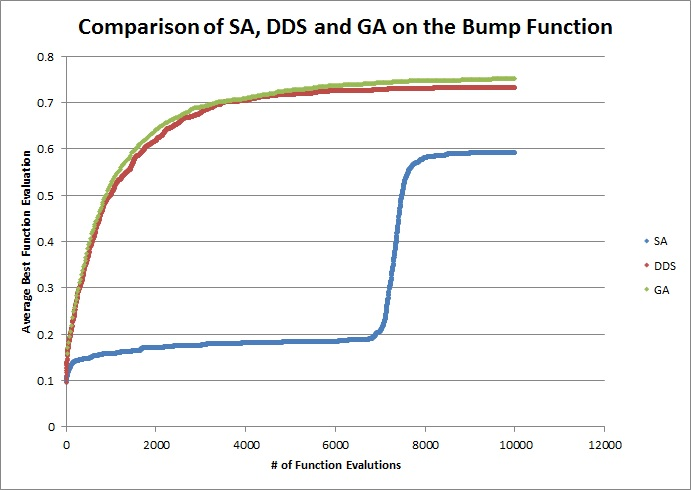
\includegraphics[scale=0.9]{abc_graph}

From the graph alone, it is clear that both GA and DDS dominate SA. It also appears that GA performs slightly better than DDS over the course of the run, and may dominate at the end.

\subsection{d}

\subsubsection{Comparison 1: Box Plot}
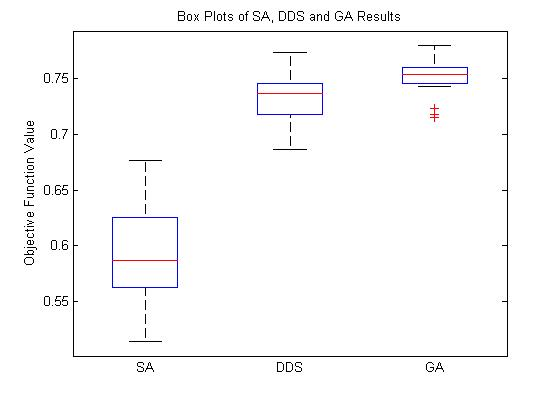
\includegraphics[scale=0.6]{boxplot}\\
\subsubsection{Comparison 2: CDF}
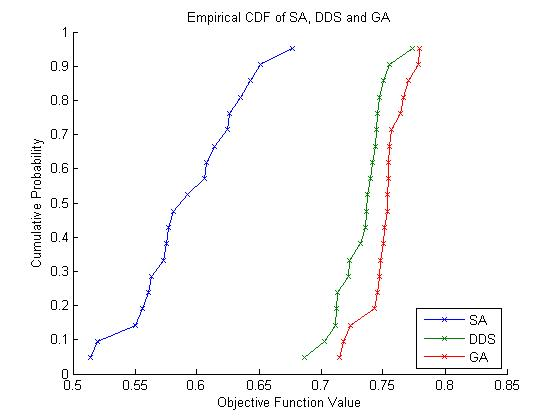
\includegraphics[scale=0.6]{cdf}\\

\subsubsection{Comparison 3: Two sample t test}

The null hypothesis for each pair is that the mean value of the two search heuristics is the same.\\\\

SA/DDS:\\\\
Statistics: T Statistic: -13.509848\\
P value for Two Sided: 0.00000\\
P value for One Sided: 0.000000\\

For comparison at $\alpha = 0.05$, $t_{\alpha/2,v} = 2.052042$, $t_{\alpha, v}  = 1.703421$. As $t < -t_{\alpha/2,v}$, we reject the null hypothesis and accept that the two mean values are different. Then, since $t <= -t_{\alpha, v}$, we can accept the alternate hypothesis that $\mu_x - \mu_y < \Delta_0$, indicating that the mean of SA is statistically significantly less than the mean of DDS.\\\\
As the means were so far off, it can easily be seen that SA performed much worse than DDS. This confirms what was seen in the graph in part c, the box plot above, and in the cdf, where DDS dominated SA.\\\\

SA/GA:\\\\
Statistics: T Statistic: -15.615549\\
P value for Two Sided: 0.000000\\
P value for One Sided: 0.000000\\

For comparison at $\alpha = 0.05$, $t_{\alpha/2,v} = 2.058272$, $t_{\alpha, v}  = 1.707344$. As $t < -t_{\alpha/2,v}$, we reject the null hypothesis and accept that the two mean values are different. Then, since $t <= -t_{\alpha, v}$, we can accept the alternate hypothesis that $\mu_x - \mu_y < \Delta_0$, indicating that the mean of SA is statistically significantly less than the mean of GA.\\\\
As the means were so far off, it can easily be seen that SA performed much worse than GA. This confirms what was seen in the graph in part c, the box plot above, and in the cdf, where GA dominated SA.\\\\

DDS/GA:\\\\
Statistics: T Statistic: -3.172571\\
P value for Two Sided: 0.003015\\
P value for One Sided: 0.001508\\

For comparison at $\alpha = 0.05$, $t_{\alpha/2,v} = 2.025410$, $t_{\alpha, v}  = 1.686598$. As $t < -t_{\alpha/2,v}$, we reject the null hypothesis and accept that the two mean values are different. Then, since $t <= -t_{\alpha, v}$, we can accept the alternate hypothesis that $\mu_x - \mu_y < \Delta_0$, indicating that the mean of SA is statistically significantly less than the mean of GA.\\\\
The means were significantly closer together in this pairing, but since both standard deviations were so low, it makes sense that we can still confirm that GA performed better than DDS. This confirms what was seen in the graph in part c, the box plot above, and in the cdf, where GA dominated DDS.


\end{document}